\chapter{绪论}

随着互联网的不断发展,以及终端设备,比如手机,拍照设备,监控设备的广泛应用,互联网上现在保存的图片数量巨大,并且每天都在以惊人的速度增长,有数据显示,2011年FaceBook上就存储了多达1000亿张图片\upcite{facebook}。如何在巨大的图像数据集中精确并且快速的找到相应的图片,逐渐发展为一个十分热门的研究课题。该问题是大数据处理及图像处理两个计算机领域问题的交叉。大数据处理技术在近年来无疑是最受关注的研究问题之一,其他的还有云计算及人工智能,三者有着紧密的联系。基于内容的图像检索技术(content-based Image Retrivel或者CBIR)\upcite{CBIR}在大数据下的图像检索(Image Retrivel)\upcite{imagerv}背景下受到研究者们的重视,该技术充分利用图片自身的信息,不需要人工的为每张图片打上描述标签,较传统的以标签搜图技术,有极大的匹配精度。现在百度\upcite{baiduPic} 和google 公司都有相应的以图搜图服务,用户通过上传相似图片,搜索系统将返回匹配成功的相似结果。CBIR技术涵盖了许多图像处理中的重要环节,比如特征提取,特征匹配等,本文的研究工作是围绕特征提取进行的。

\section{研究背景}
本小节先介绍图像检索的基本概念,然后给出两种图像检索技术的实例,分别是基于文本的图像检索(TBIR)和基于图像内容检索(CBIR)。本文对两种技术进行比较,分析各自的优点和缺点,展现CBIR的存在意义及价值,最后对海量图像内容检索中的关键步骤展开分析。

\subsection{图像检索}
在1970时就出现了图像检索技术\upcite{imagerv},当时主要还是通过输入检索文字的方式来进行图片的搜索,比如Getty AAT\upcite{GettyAAT},使用了13300个词汇来描述其下的所有图片,包括历史的,艺术的,建筑的等不同领域的图片。又如 Gograph,将其下的图片分为了30多级的检索主目录,每级目录下有含有子目录,层层递归,来划分图片的不同归类,以便于人们进行查找。上面两个例子就是以典型的文本的方式来进行图片检索的例子。

得益于研究者们的大量研究贡献,以文本的图片检索技术发展十分迅猛,现在已经有相当多的这种方式下的检索算法,比如RageRank\upcite{PageRank}算法,聚类\upcite{TextClustering}算法,语言解析算法等等,但是因为受到描述词汇的限制,描述词汇的模糊和多义性,在大数据背景下的图片检索,文本方式的图片检索效果并不理想。为了更加准确的表达搜索的意图,更加精确的搜索目标图片,基于内容的图像检索(Content-based Image Retrieval)\upcite{CBIR}技术逐渐被研究者们重视起来。

CBIR技术和TBIR技术是两种不一样的检索技术,基于内容的图像检索技术利用图片自身的信息,这里的信息可以是图片的颜色,图片的形状或者图片的纹理,同时特征可以是全局的,也可以是局部的,该技术利用上述的这些特征,然后是相应的匹配算法去查找目标图像。因为查找的信息十分精确,没有描述模糊,描述歧义等限制,因此如果提取的特征的精度和匹配算法精度同时很高,那么CBIR技术的查询返回的结果非常准确。但是由于图片的特征信息量大,因此查找的速度也会受到其制约。目前,已经存在有基于内容图像检索的商用系统,比如QBIC系统\upcite{QBIC},WebSeek系统\upcite{webseek},PhotoBook系统\upcite{Photobook},百度公司研发的百度图片系统及谷歌公司研发的google picture等。CBIR系统的运行原理架构如图\ref{fig:CBIR_fw}所示:
\begin{figure}[htp]
\centering
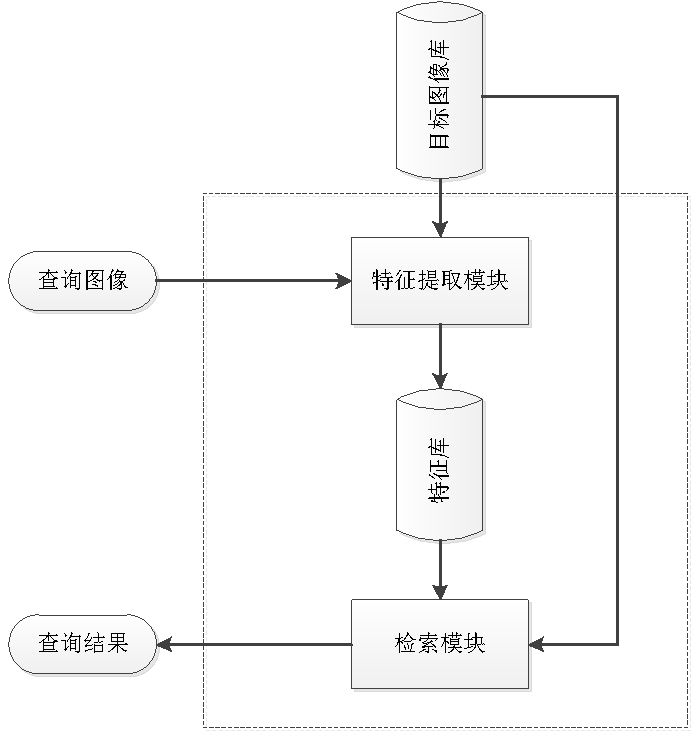
\includegraphics{retrivelfw}
\caption{基于内容的图像检索框架}
\label{fig:CBIR_fw}
\end{figure}
\\先将系统的图像库通过特征提取模块提取图片特征,然后所有被提取的特征将组成系统的特征库模块,查询图片先通过特征提取模块进行特征提取,然后将查询图片的特征和特征库中特征进行匹配,最后返回匹配的结果。

上面运行步骤中,特征提取,特征匹配是CBIR中十分重要的步骤,其中特征提取最为重要,因为如果特征提取做的不好,会直接影响后面的所有步骤,因此如果快速并且提取高质量的图像特征,一直是研究的热点。

\subsection{特征提取}
因为在计算机中,我们输入处理的都是二进制数字信号,为了使计算机能够”理解“图像,我们必须从中抽取有用的信息,得到图像的”非图像“表示或描述,比如数值,向量或者是符号,从图像到数字符号的过程就是图像的特征提取。
\subsubsection{特征分类}
全局特征和局部特征是现在图像特征的大体分类,目前对于图像特征没有很明确的定义。常见的全局特征有图片颜色信息,纹理信息,轮廓形状信息,全局特征可以较好的理解图片的总体信息及内容,但是却不太适合进行图片的匹配工作,比如一张图片为红色,如果使用红色这一特征进行匹配,那么很可能搜到许多符合条件的图片。相反局部特征就很好的胜任图片匹配这一工作。常见的局部特征有,图像的斑点信息,图像的角点信息,图片的边缘信息及图片中的脊,局部特征是一张图片中具有局部不变性的,具有图片强烈代表性的局部信息,这些信息即使在图片受到光照,遮挡,旋转等外界影响的情况,也能很好的表示图像的独特性。因此局部特征较好的应用于图像的匹配工作,而不太适合从整体上理解图像,本文研究的SIFT 算法就是一种局部特征的提取算法。以下是一些常见的全局及局部特征的定义解释:
\begin{itemize}
\item 颜色特征\\颜色特征\upcite{HSVColor1, HSVColor2}是物体表面特性的描述,归类为全局特征。由于颜色特征没有很好的捕捉物体的局部特性,因此当在一个很大的数据库中,使用颜色特征进行图像匹配时,会检出很多满足要求的结果。颜色特征的优点在于其不受物体大小尺寸变化及物体空间位移变化的影响。
\item 纹理特征\\纹理特征\upcite{TextureFeature, TextureFeature2}也是一种全局特征,和颜色特征相同的是,纹理特征也是一种图像物体表面的特性。纹理特征是对一个区域中的像素进行数学上的统计,根据统计的结果,代表图像的纹理信息。这种方式就和颜色特征提取的方式不一样,因为不是针对单个像素的。物体发生旋转时是不会影响物体的纹理特征提取,说明纹理特征可以对抗位置旋转噪声。纹理特征的缺点在于很容易受到分辨率及光照的影响,同时3D 物体投射成2D 时的纹理特征可能会发生变化。
\item 形状特征\\各种基于形状特征\upcite{ShapeFeature}的检索方法可以任意选取图像中的区域形状进行检索,简单快捷。但是该特征有几个缺陷,第一是该提取方法现在还没有完整的数学模型,因此是没有严格的数学意义上的等式证明,可能会存在不严谨性。第二当物体发生了一定形变时,基于形状特征进行匹配时就会失效,但是现实生活中物体的外部形状很可能发生变化,最简单的就是热胀冷缩。第三,3D 物体进行平面投射成2D 时,由于视觉的变化,物体的轮廓形状是发生变化的,因此对2D物体形状进行的特征提取得到的信息有可能和对同一个物体3D形态下的特征提取信息不一致,在一定程度上已经发生了失真。
\item 空间关系特征\\空间关系特征是一种全局特征,它描述了图片中物体和物体间的空间关系,空间关系可以是邻接,可以是重叠,也可以是包含等,通过空间特征关系,我们就可以对图片中物体的整体位置关系有一个主体的框架。绝对的以及相对的空间关系是对物体间空间位置信息的两种归类。绝对空间关系描述的是物体间的绝对位置关系,通过绝对空间关系特征,我们可以描述出目标和目标间的距离大小以及方位。而相对空间关系特征描述的是物体间的相对位置信息,比如是A和B在空间中是上下关系,或者是A和B是左右关系等。相对和绝对空间关系是有一定关系的,比如我们可以通过两个物体的绝对关系推算出物体间的相对关系,但是反过来则不能。空间关系特征的优点在于可以很直观的理解整幅图片的物体的空间关系,但是空间关系特征相对简单,信息量小,对物体旋转,偏移,尺度变化等噪声抵抗力不好。如果图像仅用空间信关系特征进行配置时,往往是不能达到一个很好的效果,因为信息过于单调,所以可以用空间关系特征结合另外的一些图像特征,比如颜色特征及纹理特征,来进行目标物体的匹配。
\item 角点 \\角点\upcite{CornPoint,CornPoint2}经常是被检测在边缘的交界处、被遮挡的边缘、纹理性很强的部分。如果提取的角点的质量非常高的话,那么使用这些角点可以十分准确的描述图像的独特性。
\item 斑点\\斑点通常是指与周围有着颜色和灰度差别的区域,如草原上的一棵树或一栋房子,一个湖泊中的一只小船。斑点是针对一个区域进行提取的,提取的特征点的质量高于角点,能更好的代表物体的独特性,所以它在图像配准上扮演了很重要的角色。SIFT算法中检测的特征点其实就是斑点,本文的研究也是在SIFT算法的基础上进行的。
\end{itemize}
\subsubsection{提取算法}
不同类型的特征对应着不同的提取算法,算法的原理不一样,提取精度不一样,计算复杂性也不一样。
\begin{itemize}
\item 颜色直方图法\upcite{ColorHistogram}\\通过将图片中的全局区域的R,G,B分量进行抽离,计算每一个分量占的比重,根据比重构造一个直方图,以上就是颜色直方图的基本原理。因为该方法是在物体的总体层次上进行统计和计算的,因此它和物体的空间关系是没有太大关系,当物体发生了旋转,尺度缩放等物理空间变化是,不是会影响颜色直方图法提取的结果的。但是正是由于它对物理位置不敏感,会导致许多图片中物体关系是完全不一致的,但是它们计算出来的颜色直方图却是一样的,这就是为什么有时候利用颜色直方图在很大的图片数据集下进行目标查找,查询结果包含许多无关的图片。
\item 灰度梯度共生矩阵\upcite{GLCM}\\ 灰度梯度共生矩阵(Gray-GradientCo-occurrence Matrix)方法是一种具有统计意义的纹理特征分析方法。该方法统计图像的梯度及灰度信息,然后使用一个矩阵保存提取到的信息。GGCM的描述方法的优势在于可以很好的描述图像灰度和梯度的变化规律,同时也很好的描述了图像的纹理特征,特别适用于具有方向性的纹理描述。灰度梯度共生矩阵是一个计算效率很好的矩阵,因为在该矩阵的基础上,还可以统计出许多其他额外的信息,比如灰度及梯度的平均数值、灰度和梯度方差数值等等,有相关的研究者\upcite{GLCM2}在研究灰度梯度共生矩阵的基础上,又提取额外的能量,惯量等四个维度的信息,精度相当高。
\item 几何法\\几何法其实也是一种针对图像纹理信息的特征提取方法。根据纹理理论,纹理信息很多时候是具有规则的几何特征的,因此可以使用几何的方法来进行图像纹理信息的提取。分别是Voronio 棋盘格特征法\upcite{VoronoiDiagrams}和结构法是几何法中很有权威性的算法,精度也十分高。
\item 边界特征法\\该算法是一种针对图像的外围轮廓形状进行提取,获取物体形状信息。在该算法领域中,有许多有代表性的算法,在这里介绍两种比较经典的算法,它们分别是Hough 变换检测平行直线方法\upcite{HoughTransform} 和边界方向直方图方法\upcite{Boundary} 。Hough 变换检测平行直线方法是将图片中物体边界处具有相同特征的点归类聚集在一起,最终将物体的外围形状轮廓提取出来。Hough 方法在物体空间参数不是很大的情况下,提取的总体效果还是很不错的。但是如果被检测的物体的体积很大,那么该算法计算的时间会很长,并且也需要开辟很大的存储空间来保存检测出来的边界特征点。边界方向直方图法其实也是利用直方图来获取物体的边界形状信息的,该方法首先会对物体边界求微分,在根据微分的结果做出一个直方图,最终获取物体的形状信息。
\item 傅里叶形状描述符法\\傅里叶形状描述符(Fourier shape deors)\upcite{Fourier}方法是对物体的外围轮廓进行Fourier变换数学运算,通过傅里叶变换函数的特性,物体的边界的连续性,边界性及封闭性均能很好的表现出来。同时傅里叶形状描述法还有降维的优点,可以将二维的物体空间转换为一维向量,从而降低了物体外围形状的时间复杂性。
\item 尺度不变特征转换法\\尺度不变特征转换(Scale-invariant feature transform或SIFT)\upcite{SIFT}是一种局部特征提取算法,该算法先对目标图像构建尺度空间,这里的尺度空间在实际计算时是用高斯金字塔作为实例,随后算法就会在整组高斯塔上去搜索特征点,这些点不是普通的点,它们是可以十分准确的将物体的独特性描述出来的,即使物体被轻度的物理改变了,最后算法将这些点提取出来,使用128维向量来在数学层次上描述一个特征点,所有提出出来的特征点就形成了被检测物体的特征点集合。SIFT 算法提出来的特征点抗噪声能力十分强大,在物体被光照,遮挡,旋转等影响因素干扰下,算法依然可以十分高的精度将物体识别出来,是一个具有划时代意义的算法。
\item Harris角点检测法\upcite{Harris}\\该算法的基本思想是,使用一个的检测窗口进行在目标检测物体进行行列扫描检测,根据移动导致周边区域的灰度变化情况来判断这个检测区域是否存在检测。通常情况下,角点一般出现在检测区域和周边区域有着十分大的灰度落差的窗口上,当确定了区域窗口,在窗口上进行更细区域的搜索。检测的窗口一般是高斯函数,即使用高斯函数和图片的固定区域不断进行卷积操作。该算法检测出来的特征角点稳定性好,可以抵抗较大的物理噪声,同时算法的计算效率也较高。
\end{itemize}

在众多的提取算法中,综合考虑了算法提取的精度,算法的时间复杂度及空间复杂度以及可以突显大数据处理框架的在大规模处理时的高效性,本文选取了SIFT算法\upcite{SIFT2}作为研究点,将其应用于大数据处理框架Spark上,完成大规模图像库的快速提取工作,本文将在第二章详细介绍SIFT 算法的原理以Spark的基本原理。

\subsection{特征匹配}
除了上述讨论的特征提取技术之外,特征匹配也是图像处理中一个很关键的处理步骤,它们相互补充,如果特征点提取不好,那么匹配算法在好也没有。反过来,如果匹配算法不够精确,提取的特征点在精确不能达到精确查找物体的目的。图像匹配问题实际就是相似搜索\upcite{SimilaritySearche} 或者是近似搜索\upcite{ProximitySearch} 问题。相似搜索是指对于给定的检索的数据对象,根据预先设置好的相似阈值,在目标的数据集合中查找所有满足要求的目标对象,阈值设置的大,返回结果的越多,反之越少。阈值就代表匹配相似度的评判准则,关键在于我们怎样去对相似度进行定义,什么维度的评判才是匹配时有价值的评判标准,常见的相似度的定义方式有下面几种:
\begin{itemize}
\item 汉明距离。给定比较的两个字符串x及y,它们的汉明距离计算如公式\ref{hanming}所示:
\begin{equation}\label{hanming}
Ha=\sum_{1}^d(x_i=y_j)
\end{equation}

\item $l_p$ 范数距离。给定d维实数空间$R_d$中的两个向量点x=($x_1$,...,$x_d$)和y=($y_1$,...,$y_d$),x和y之间$l_p$-范数距离的计算表达式如下:
\begin{equation}\label{fanshu}
L_p(x_i,y_i)=\Bigl(\sum_{l=1}^n(x_i-y_i)^p\Bigr)^\frac{1}{p}
\end{equation}

\item 余弦距离。给定x和y,它们是d维实数空间$R_d$中两个非零向量,那么它们的余弦距离计算公式如下:
\begin{equation}\label{yuxian}
\cos(x,y)=\frac{xy}{|x|_2|y|_2}
\end{equation}

\item Jaccard距离。给定两个集合A和B,它们之间的Jaccard距离的计算公式如下:
\begin{equation}\label{Jaccard}
Ja(A,B)=\frac{|{A}\cap{B}|}{|{A}\cup{B}|}
\end{equation}
\end{itemize}

特征向量的维度越高,特征的描述也越详细,匹配的精度也就越高,如常见的sift特征是128维,Gist特征是960维,深度学习提取的特征维度是1024维甚至更高。在面对着这些高维的特征向量时,如果完全单纯的计算每个向量间的距离,匹配速度将会十分缓慢,因此研究者们想追求的肯定是在匹配的精度很高,同时匹配的速度要很快,虽然很多时候我们要么割舍精度来换速度或者是降低速度来换取精度。面对高维特征向量,可以通过给特征建立有效的索引来提升查询效率,比如KD-tree\upcite{KDTree},R-Tree\upcite{RTree}或者SR-tree\upcite{SRtree} 等,这些方法的基本思想是将有相同特性或者是相近的特性的特征点统一划分到一个区域上,然后给这个区域建立一个索引,查找时根据索引先确定某个区域,然后再在区域中进一步查找,从而提升查找的效率。建立索引方式在面对着超高维特征向量时,效率还是偏低,有学者提出了降维的思想,将超高维向量降低到某个维度,牺牲部分精度来大幅度提升查询效率,这种思想的最著名实现就是局部敏感哈希算法\upcite{LSH},该方法通过适当的调节参数,可以保证很高的精确度条件下也有很高的查询效率。

特征匹配方法在本设计工作中只是充当验证特征提取正确性的角色,并不是研究的重点,因此在第二章的基本原理部分没有对特征匹配进行深入的原理分析。

\subsection{大数据处理处理技术}
如今社会中的数字信息越来越多,各行各业现在都面临着大数据北京下数据处理的技术挑战,无论是处理的数据规模,还是处理的数据的速度,单台机器早已无法满足当今大数据应用的处理要求了,因此我们需要有一个大数据背景下的数据处理或者是存储框架,以帮助我们更加轻松的处理海量数据。自从谷歌公司提出了大数据的概念以及发表的三篇奠定大数据框架的论文之后,很多大数据处理框架在此基础下不断诞生。接下来,本文将会介绍内存计算引擎Spark 和分布式文件系统HDFS 两个大数据处理框架,它们分别是本文设计工作中的计算引擎以及数据存储核心层。
\subsubsection{内存计算框架spark}
Apache Spark 是专门为大规模数据处理而设计的快速通用的计算引擎,它的开发者为UC Berkeley AMP lab (加州大学伯克利分校的AMP实验室)。Spark的最大特点在于其内存持久化技术,可以将计算过程中的中间结果保存到内存,大大提升了计算任务的运算速率,十分适合迭代次数多的作业,比如像大规模图计算作业,神经网络作业等。Spark本质还是Mapreduce框架,这点和Hadoop是相同,在MapReduce框架下,计算任务Map Task 被分发到Slave上,计算结束后,通过Reduce Task 统一收集Master上或者保存到HDFS中,区别还是在于Spark的中间结果支持内存缓存机制。Spark提供了一套完成的内存编程模型及容错重算机制,使得开发者可以像编写普通程序一样去编写内存作业的应用程序,也不用担心缓存在内存的中间结果因为某些原因而丢失。

除了Map和Reduce操作之外,Spark还提供了丰富的生态应用环境,比如提供了SQL与结构化数据处理工具Spark SQL,机器学习工具MLib,分布式图计算引擎Graphx以及流式处理工具Spark Streaming。同时Spark的编程接口十分丰富,支持Scala,java,Python和R语言。Spark框架如图~\ref{fig:sparkfw}所示:
\begin{figure}[htp]
\centering
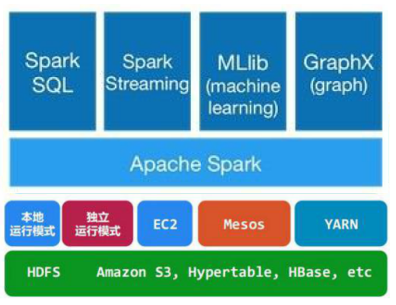
\includegraphics{sparkfw}
\caption{spark框架}
\label{fig:sparkfw}
\end{figure}

Spark的核心是RDD(Resilient Distributed Datasets)\upcite{Spark},RDD是一个分布式内存数据结构,可以将内存存储透明化,让用户显式地将数据存储到磁盘和内存中,并能控制数据的分区。RDD的编程接口非常丰富,基本可以满足所有常见开发的需求。RDD的接口操作也成为算子,比如Map算子,FlatMap算子,filter算子,这些算子都是monad模式的算子,即是不带key特性的单边数据处理。同时Spark的RDD接口中也提供了丰富的Key特性处理接口,比如join,groupByKey,reduceByKey等算子。通过Spark下这些内存运行运算算子,我们可以很容易的实现单机到分布式的功能转换。

在本文的设计工作中,我们将Spark作为大规模图像特征提取的计算引擎,加速特征提取的工作。
\subsubsection{分布式文件系统HDFS}
在BigData背景下,需要被处理数据的规模往往是非常大的,很多时候达到了TB级别的,传统的单机的数据存储方式是无法满足读写速度要求及数据存储可靠性,这这种情况下,需要一种数据的分布式存储方案,将处理的数据分散存储而有集中管理,分布式文件系统HDFS就是这样的一种存储方案。虽然现在已有的网络文件系统(NFS)也算是一种分布式存储解决方案,但是相比之下,HDFS存储方案的执行效率及安全性,是要远高于传统的的NFS 架构。因为NFS 本质上还是单机的存储方式,只不过访问端和存储端是处于分布式的状态,一旦客户端的访问量过大,就会造成服务端拥堵。而次,NFS的安全可靠性也不如HDFS,在HDFS的有完整的大数据场景下的文件备份方案,保证某个节点数据损坏后,可以迅速恢复。在数据的同步性上,HDFS的效率会高于NFS,因为在NFS下,客户端的写操作必须要先上传服务端,其他的客户端才能感知到数据的修改,在HDFS 下则不需要先经过服务器端这一操作。

HDFS,是Hadoop Distributed File System的简称,是Hadoop抽象文件系统的一种实现。HDFS是Google大数据三大论文中《The Google File System》\upcite{HDFS}的实现。整个HDFS 集群有Namenode 和Datanode构成master-worker(主从)模式。Namenode复杂构建命名空间,存储Mete数据,而Datanode则存储data数据。HDFS整体框架图~\ref{fig:hdfsfw}所示:
\begin{figure}[htp]
\centering
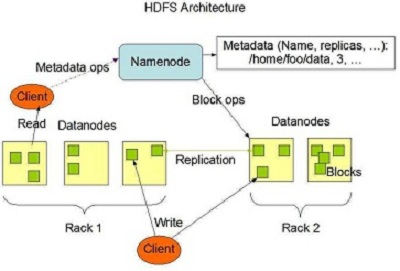
\includegraphics{hdfsfw}
\caption{hdfs框架}
\label{fig:hdfsfw}
\end{figure}

HDFS在本文的设计中起分布式存储的作用,系统中的原始图像库,序列化图像库,特征库以及运行日志都保存在HDFS中。

\section{研究问题及研究现状}
本文研究的重点是如何加速大规模图像数据集的特征提取技术,因为根据之前分析,该技术在内容检索中的最为重要,并且耗时十分长,因此该研究问题实际意义十分强。

关于图像特征提取问题的研究,很早就有学者开展研究了,而特征提取发展中具有里程碑式的工作应当是Lowe等人在2000年提出的SIFT算法,该算法具有局部不变的特性,意味着在物体被旋转或者是被遮挡的情况下,都不会影响图像的识别,并且算法对光线、噪声、微视角改变的容忍度也相当高。如果这些特征点进行匹配工作,即使是检索的图像数据集很大,也能很精确的查找出目标物体。但是由于SIFT算法时间复杂性高,特征提取时间难以满足实时要求,后续有大量学者在SIFT算法的基础上做优化工作,以提高特征提取的时间。

目前针对SIFT算法性能优化的工作主要体现在两个方面,一是在算法数字本质的基础上改进算法以降低时间开销、提高特征提取速度。例如Bay提出SURF(Speeded Up Robust Features)\upcite{SURF}延续SIFT算法的思想,通过积分图像和Haar 小波相结合大大的提升了特征提取的速率;Ethan R.等人提出的ORB算法\upcite{ORB}采用了一种快速的基于Brief的二进制特征描述子方法提高了特征检测速度;Matas 等人则提出了最大极值区域(MSERS, Maximally stable Extremal Regions)特征检测方法\upcite{MSERS},MSERS检测图像中灰度最稳定的区域,然后对检测区域进行旋转和尺度的归一。二是借助FPGA、GPU等硬件加速器提高SIFT算法的性能,例如S.Heyman 等人将SIFT算法移植到GPU上\upcite{GPUSIFT},获得了不错的性能加速。本文则研究了基于Spark 优化SIFT 算法性能的方法。

在大数据和图像处理的交叉研究中,也有许多出色的研究工作,例如,Hadong Zhu 等和Akash K Sabarad 等分别在Hadoop 平台下实现了大规模图像特征提取\upcite{HadoopImage1,HadoopImage2},相对于单机环境,获得了不错的加速比;Hanli Wang等设计了一个云平台下的大规模图像检索的处理框架CHCF\upcite{HadoopImage3},Manimala Singha 等基于Hadoop 设计并实现了一个基于内容检索的图像检索框架\upcite{HadoopImage5}。 和上述工作不同的是,本文是基于Spark下进行图像处理技术的研究。

大数据处理框架Spark自在Apach上开源以来,一直都受到热烈的关注,有许多研究者都使用Spark进行数据的处理,包括现在十分火热的机器学习,深度学习都有在Spark上应用,比如基于Spark的机器学习库MLib\upcite{Mlib},将Spark和deep learning 结合的进行移动数据分析和研究\upcite{SparkDeepLearing},基于Spark的对规模图计算\upcite{SparkGraph},但是我们发现Spark现在更多的是进行纯文本的分析,直接对图像进行处理的尚未发现,并且Spark 里面也没有对图像处理支持的相关库,因此这也促使我们产生在Spark 上进行图像处理的相关研究,因此我们就选取了图像处理中的特征提取步骤,在Spark 上开展研究。

\section{本文工作与成果}
\begin{figure}[htp]
\centering
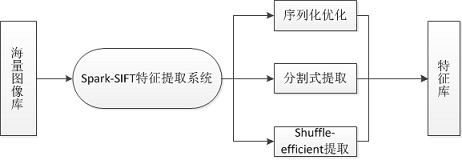
\includegraphics{workfw}
\caption{工作成果展示}
\label{fig:workfw}
\end{figure}
如图~\ref{fig:workfw}所示,针对大规模图像特征提取,我们设计了一个基于Spark大规模图像特征提取系统Spark-SIFT,然后,我们针对该系统提出了三种优化方案。首先,我们针对单个图片体积较少,而HDFS读写小文件效率又不高问题,我们对系统进行了序列化优化。然后,针对Spark现有的任务划分方式造成的负载不均衡问题,我们提出了分割式的特征提取算法。最后,我们针对分割式算法的基础上,进一步优化,提出了Shuffle-efficient 的特征提取算法。具体研究内容概括如下:
\begin{compactenum}
\item 大规模图像库分布式提取系统Spark-SIFT\\本文首先实现了一个Spark下的图像处理基础库SparkImgLib,然后基于SparkImgLib,本文实现了Spark 框架下的SIFT算法,再在Spark-sift算法上的基础上,本文有实现了一个大规模的图像库特征提取系统。
\item key-value图片描述是数据结构\\spark在加载众多小文件时性能较低,而处理的图片体积一般是比较小的,比如几百K,因此本文设计中采用用key-value的方式描述一张图片,将图片以record 的形式序列化保存到HDFS 中,从而使得Spark可以一次性加载多条记录,提升了读写的性能。
\item 分割式特征提取算法\\Spark在进行任务划分时只考虑了task总体积,但是这种划分方式在本文设计中可能会造成tasks的负载不均衡,因为图片本身大小也会影响tasks的运行时间,针对这一点,我们提成了分割式的图片特征提取算法,将较大的图片分割成子块,来改善Spark在因为tasks划分方式导致的负载不均衡问题。
\item Shuffle-efficient特征提取算法\\Spark中Shuffle机制是影响性能的重要因素。分割式提取算法中存在Shuffle问题,比如同一图片的子块散落在不同的分区时的数据混洗以及在不同分区上收集同一张图片子块时的数据混洗。针对上述Shuffle问题,我们提出了shuffle-efficient的特征提取算法,提升shuffle性能。
\end{compactenum}

\section{论文结构}
本文一共分为6个章节,总体结构如图~\ref{fig:paperfw}所示:
\begin{figure}[htp]
\centering
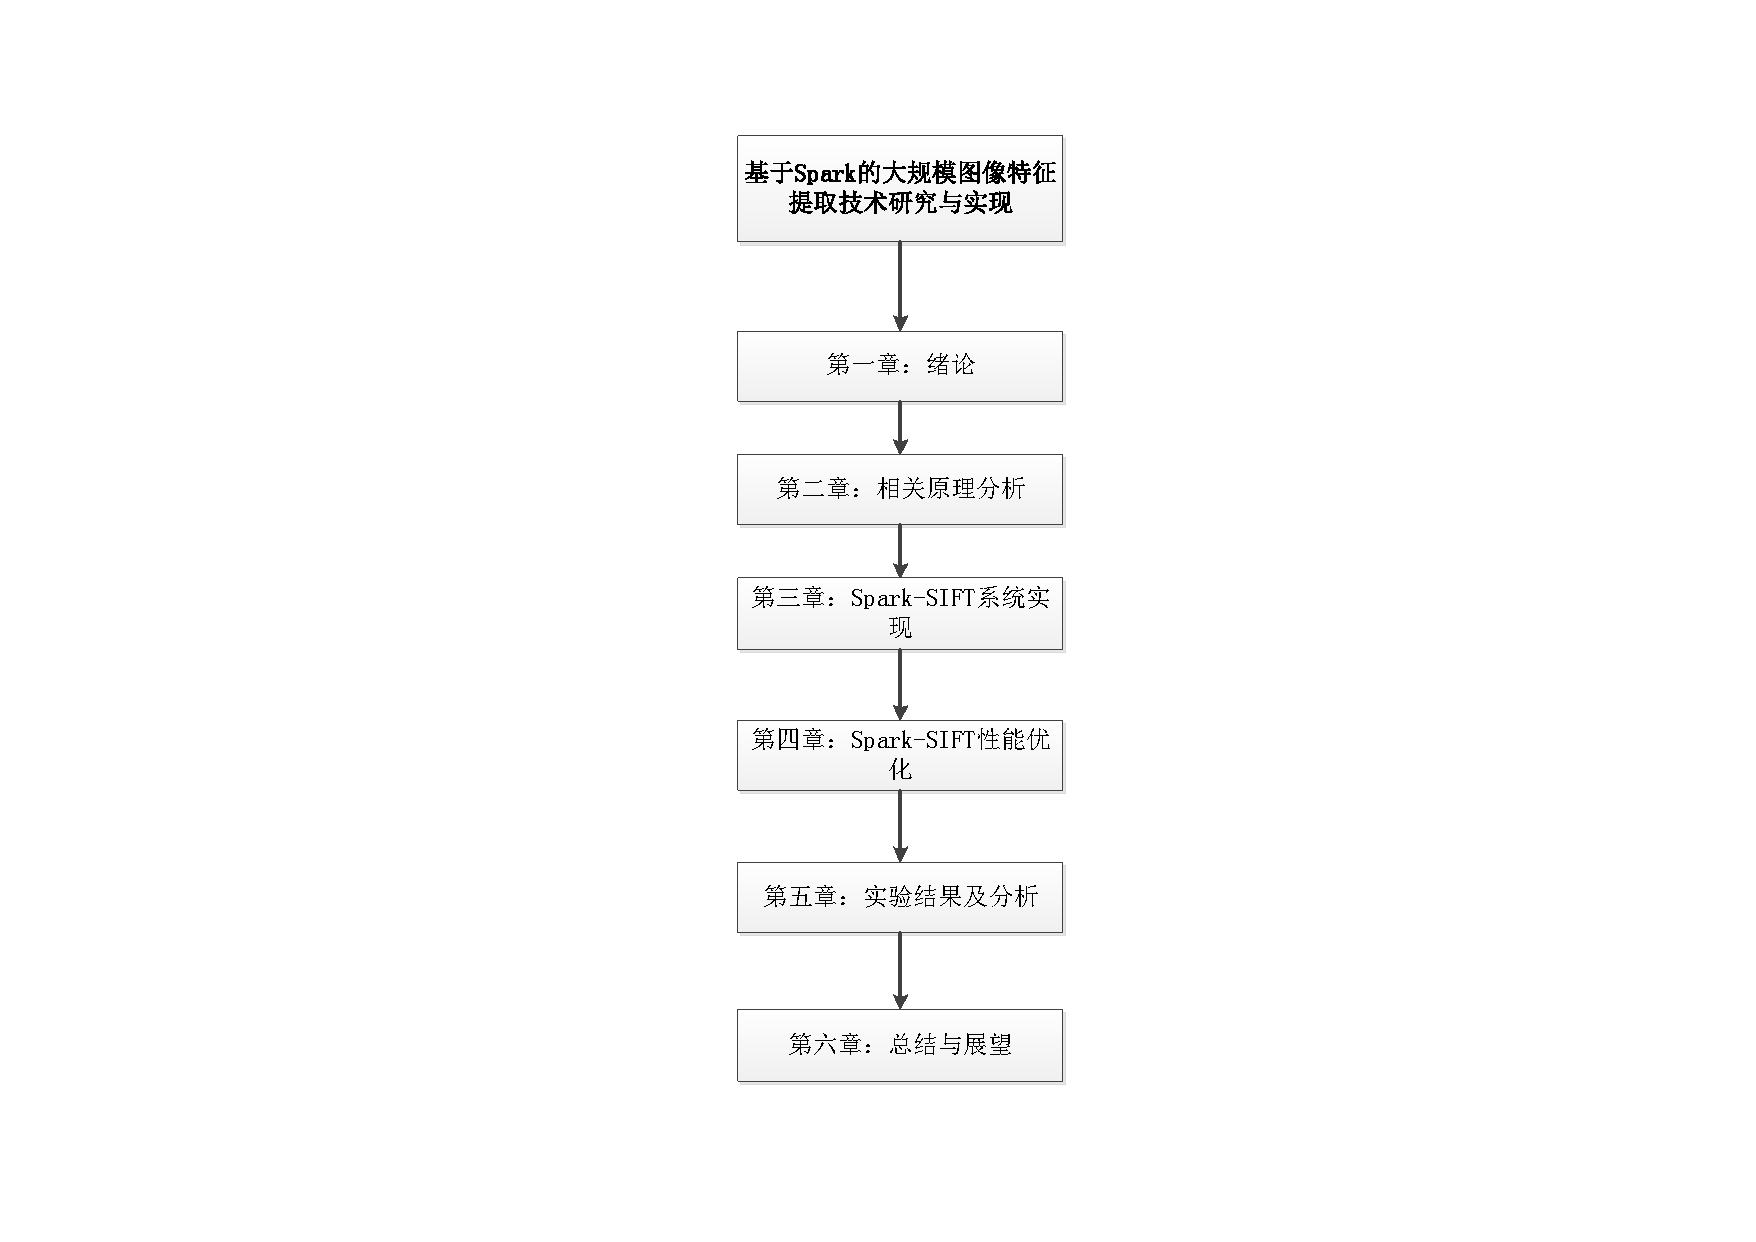
\includegraphics{paperfw}
\caption{论文组织结构}
\label{fig:paperfw}
\end{figure}

第一章为绪论,在绪论中,我们首先讨论了TBIR技术和CBIR技术的区别,分析了两者的优缺点及使用场景,通过对别突显了CBIR技术存在意义,进而引出了CBIR中的两个关键技术,分别是图像特征提取技术和图像匹配技术。对于特征提取部分,本文首先对常见的特征进行分类,解释每一种的定义及区别,接着又针对不同类别的特征给出相应的特征提取方法。对于特征匹配部分,我们解释了匹配的基本原理及几种度量方式的特点和区别。在介绍完CBIR关键处理技术后,我们分析了对本文设计工作中所涉及到到的大数据处理技术,在这部分内容中,我们主要介绍了本系统设计中的两个大数据处理框架Spark和HDFS,我们分析了它们的存在的价值,技术特点,及在本文设计中扮演的角色。最后,介绍了本文的研究问题及问题研究现状,本文工作成果以及论文结构三部分。

第二章本文分析了设计中所涉及的一些原理知识,这些知识为本文的设计工作提供理论基础。

第三章介绍了大规模图像库特征提取系统Spark-SIFT系统的整体设计工作,先介绍整个Spark-SIFT系统的整体框架,然后针对框架中的每个模块,包括序列化预处理模块,分布式特征模块,分布式存储模块等进行详细的分析。

第四章介绍了在Spark-SIFT基础上提出的三种优化方案,分别是key-value的图片描述方式,分割式特征提取算法以及shuffle-efficient特征提取算法。

第五章进行性能数据的分析,分别针对Spark-SIFT系统的三种优化策略性能以及Spark-SIFT系统的综合性能进行对别分析

第六章总结了本文的所有设计工作及创新点,分析了存在的不足点,最后对未来工作的一些看法和展望。


